\documentclass[a4paper, 11pt]{article}

% -- Coments
\usepackage{verbatim}

% ----- Fonts -----
% -- Fuente --
% \usepackage{fontspec}
% \setmonofont{JetBrainsMono Nerd Font}  

% -- Color --
\usepackage{xcolor}
%\definecolor{azul}{RGB}{00,33,99}
\definecolor{azul}{RGB}{35,72,180}

% -- Page Margin --
\usepackage[margin=1in]{geometry}

% -- Espaciados --
\newcommand{\Pspace}{0.5cm}
\newcommand{\Aspace}{0.2cm}

% -- Columnas --
\usepackage{multicol}

% -- Imagenes --
\usepackage{graphicx}
\usepackage{float}

% -- Matemáticas --
\usepackage{amsmath, amssymb}

% -- Gráficas --
\usepackage{pgfplots}
\pgfplotsset{compat=1.18}

% -- Código --
\usepackage{listings}
\lstset{
    language=C++,                   % Lenguaje del código
    basicstyle=\ttfamily\small,     % Fuente del código
    keywordstyle=\color{blue},      % Color de palabras clave
    commentstyle=\color{gray},      % Color de comentarios
    stringstyle=\color{red},        % Color de cadenas
    numbers=left,                   % Números de línea a la izquierda
    numberstyle=\tiny\color{gray},
    breaklines=true,                % Permitir saltos de línea
    frame=single                    % Marco alrededor del código
}

\begin{comment}
-- Formato de pregunta simple
    % - Problema n
    \vspace{\Pspace}
    \item Problema \par
        % Respuesta:
        \vspace{\Aspace} \par
        { \color{azul}  }


 -- Formato de pregunta multimple
        % - Problema 
        \vspace{\Pspace}
        \item  \par
             % Respuestas:
            \vspace{\Aspace} \par
            a) 
            \\ { \color{azul} }

            \vspace{\Aspace} \par
            b) 
            \\ { \color{azul} }


 -- Formato de imagen
\begin{figure}[!ht]
    \centering
    \includegraphics[width=0.5\textwidth]{}
\end{figure}


 -- Formato de tabla
\begin{tabular}{c|c}
    \textbf{A} & \textbf{B} \\
    \hline
    Texto & Texto \\
    Texto & Texto
\end{tabular} \\
\end{comment}


\title
{
    Sistemas Operativos 2026-2 \\
    Round Robin
}

\begin{document}

\maketitle

\begin{center}
    \begin{tabular}{r|l}
        \textbf{Expediente} & \textbf{Nombre} \\ \hline
        219208106 & Bórquez Guerrero Angel Fernando \\
    \end{tabular}
\end{center}

\rule{\linewidth}{0.3mm}

\vspace{0.3cm}
\begin{enumerate}
    \item Ejemplo de RR con $q = 20$: \par
    \begin{tabular}{|c|c|}
        \hline
        \textbf{Procesos} & \textbf{Periodos de CPU} \\
        \hline
        P1 & 53 \\
        \hline
        P2 & 17 \\
        \hline
        P3 & 68 \\
        \hline        
        P4 & 24 \\
        \hline
    \end{tabular} \\
\begin{center}
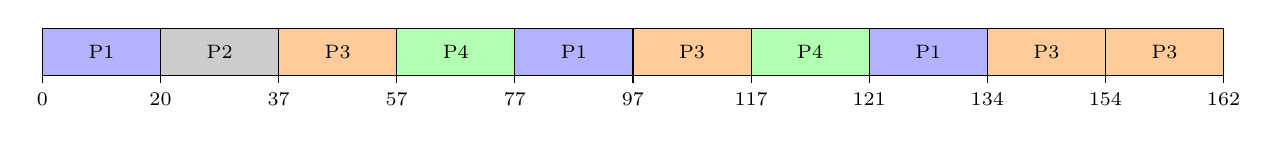
\begin{tikzpicture}[x=1.5cm, y=1cm]
  \draw[fill=blue!30, thin] (0,0) rectangle (1,0.6);
  \node at (0.5,0.3) {\scriptsize P1};
  \draw[fill=gray!40, thin] (1,0) rectangle (2,0.6);
  \node at (1.5,0.3) {\scriptsize P2};
  \draw[fill=orange!40, thin] (2,0) rectangle (3,0.6);
  \node at (2.5,0.3) {\scriptsize P3};
  \draw[fill=green!30, thin] (3,0) rectangle (4,0.6);
  \node at (3.5,0.3) {\scriptsize P4};
  \draw[fill=blue!30, thin] (4,0) rectangle (5,0.6);
  \node at (4.5,0.3) {\scriptsize P1};
  \draw[fill=orange!40, thin] (5,0) rectangle (6,0.6);
  \node at (5.5,0.3) {\scriptsize P3};
  \draw[fill=green!30, thin] (6,0) rectangle (7,0.6);
  \node at (6.5,0.3) {\scriptsize P4};
  \draw[fill=blue!30, thin] (7,0) rectangle (8,0.6);
  \node at (7.5,0.3) {\scriptsize P1};
  \draw[fill=orange!40, thin] (8,0) rectangle (9,0.6);
  \node at (8.5,0.3) {\scriptsize P3};
  \draw[fill=orange!40, thin] (9,0) rectangle (10,0.6);
  \node at (9.5,0.3) {\scriptsize P3};
  \draw[thin] (0,0) -- (10,0);
  \draw[thin] (0,0) -- (0,-0.1) node[below] {\scriptsize 0};
  \draw[thin] (1,0) -- (1,-0.1) node[below] {\scriptsize 20};
  \draw[thin] (2,0) -- (2,-0.1) node[below] {\scriptsize 37};
  \draw[thin] (3,0) -- (3,-0.1) node[below] {\scriptsize 57};
  \draw[thin] (4,0) -- (4,-0.1) node[below] {\scriptsize 77};
  \draw[thin] (5,0) -- (5,-0.1) node[below] {\scriptsize 97};
  \draw[thin] (6,0) -- (6,-0.1) node[below] {\scriptsize 117};
  \draw[thin] (7,0) -- (7,-0.1) node[below] {\scriptsize 121};
  \draw[thin] (8,0) -- (8,-0.1) node[below] {\scriptsize 134};
  \draw[thin] (9,0) -- (9,-0.1) node[below] {\scriptsize 154};
  \draw[thin] (10,0) -- (10,-0.1) node[below] {\scriptsize 162};
\end{tikzpicture}
\\[2pt] {\footnotesize\color{black} Figura 1. Diagrama de Gantt de la ejecución de los procesos.}
\end{center}
    RR TIEMPO DE ESPERA PROMEDIO = 73 \\
    SJF T.E. Promeido = 38 \\
    FCFS T.E. Promedio = 65.25
        % Respuestas:
        \vspace{\Aspace} \par
        Calcular un valor de q  para reducir el tiempo de espera promedio para el algoritmo de Round Robin
        \par { \color{azul} 
        \textbf{Planteamiento.} Con todos los procesos presentes en $t=0$ y sin considerar el costo del cambio de contexto, el tiempo de espera de cada proceso es
        \[ W_i = (\text{tiempo de finalización}) - (\text{CPU burst}). \]
        Con $q=20$ los procesos terminan en $P_1=134$, $P_2=37$, $P_3=162$ y $P_4=121$, de modo que $W = (81+20+94+97)/4 = 73$, que coincide con el valor dado.

        \textbf{Búsqueda de $q$.} Se simuló Round Robin para todos los valores enteros $q=1,\dots,100$ y se calculó el tiempo de espera promedio en cada caso. Algunos de los resultados:

        \begin{center}
        \begin{tabular}{|c|c|c|c|c|c|c|c|c|c|}
            \hline
            $q$ & 9 & 18 & 20 & 24 & \textbf{27} & 30 & 53 & $\ge 68$ \\
            \hline
            $\overline{W}$ & 71.75 & 69.5 & 73 & 68 & \textbf{65} & 68 & 67.5 & 65.25 \\
            \hline
        \end{tabular}
        \end{center}

        El mínimo se obtiene con $\boldsymbol{q = 27}$, con un tiempo de espera promedio de $65$.

        \textbf{¿Por qué $q=27$?} Los procesos cortos $P_2$ (17) y $P_4$ (24) terminan en su primer turno siempre que $q \ge 24$. Por su parte, $P_1$ (53) necesita tres turnos si $q<27$, pero solo dos si $q \ge 27$, porque $\lceil 53/27 \rceil = 2$. Entonces $27$ es el valor más pequeño con el que todos terminan en el mínimo de turnos posible. Si $q$ crece más, ningún proceso termina antes y solo se retrasa a los demás: de $q=27$ a $q=52$ el promedio sube una unidad por cada unidad de $q$.

        \textbf{Ejecución con $q=27$:}
\begin{center}
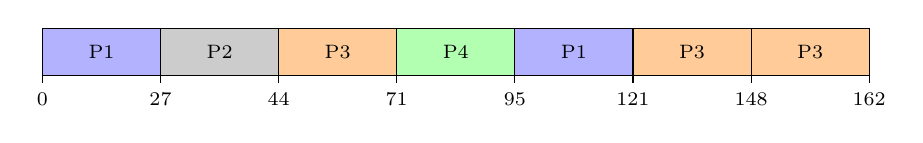
\begin{tikzpicture}[x=1.5cm, y=1cm]
  \draw[fill=blue!30, thin] (0,0) rectangle (1,0.6);
  \node at (0.5,0.3) {\scriptsize P1};
  \draw[fill=gray!40, thin] (1,0) rectangle (2,0.6);
  \node at (1.5,0.3) {\scriptsize P2};
  \draw[fill=orange!40, thin] (2,0) rectangle (3,0.6);
  \node at (2.5,0.3) {\scriptsize P3};
  \draw[fill=green!30, thin] (3,0) rectangle (4,0.6);
  \node at (3.5,0.3) {\scriptsize P4};
  \draw[fill=blue!30, thin] (4,0) rectangle (5,0.6);
  \node at (4.5,0.3) {\scriptsize P1};
  \draw[fill=orange!40, thin] (5,0) rectangle (6,0.6);
  \node at (5.5,0.3) {\scriptsize P3};
  \draw[fill=orange!40, thin] (6,0) rectangle (7,0.6);
  \node at (6.5,0.3) {\scriptsize P3};
  \draw[thin] (0,0) -- (7,0);
  \draw[thin] (0,0) -- (0,-0.1) node[below] {\scriptsize 0};
  \draw[thin] (1,0) -- (1,-0.1) node[below] {\scriptsize 27};
  \draw[thin] (2,0) -- (2,-0.1) node[below] {\scriptsize 44};
  \draw[thin] (3,0) -- (3,-0.1) node[below] {\scriptsize 71};
  \draw[thin] (4,0) -- (4,-0.1) node[below] {\scriptsize 95};
  \draw[thin] (5,0) -- (5,-0.1) node[below] {\scriptsize 121};
  \draw[thin] (6,0) -- (6,-0.1) node[below] {\scriptsize 148};
  \draw[thin] (7,0) -- (7,-0.1) node[below] {\scriptsize 162};
\end{tikzpicture}
\\[2pt] {\footnotesize\color{black} Figura 2. Diagrama de Gantt con Round Robin y $q = 27$.}
\end{center}
        \begin{center}
        \begin{tabular}{|c|c|c|c|}
            \hline
            \textbf{Proceso} & \textbf{CPU burst} & \textbf{Finaliza en} & \textbf{Espera} $= $ fin $-$ burst \\
            \hline
            P1 & 53 & 121 & $121-53 = 68$ \\
            \hline
            P2 & 17 & 44 & $44-17 = 27$ \\
            \hline
            P3 & 68 & 162 & $162-68 = 94$ \\
            \hline
            P4 & 24 & 95 & $95-24 = 71$ \\
            \hline
        \end{tabular}
        \end{center}
        \[ \overline{W}_{RR,\,q=27} = \frac{68+27+94+71}{4} = \frac{260}{4} = 65 \]

        \textbf{Conclusión.} Con $q=27$ el tiempo de espera promedio baja de $73$ (con $q=20$) a $65$, una mejora de 8 unidades (aprox.\ 11\,\%). También queda ligeramente por debajo de FCFS ($65.25$), pero no alcanza a SJF ($38$), que es el óptimo en tiempo de espera promedio. En la práctica, un $q$ muy pequeño aumentaría la sobrecarga por cambios de contexto, por lo que un valor como $27$ también es razonable en ese sentido.

        }
\end{enumerate}
\end{document}
